\begin{frame}
	\myheading{Module 8.7 : Adding Noise to the inputs}
\end{frame}

\begin{frame}
	\vspace{4em}
	\begin{overlayarea}{\textwidth}{\textheight}
		\begin{block}{Other forms of regularization}
			\begin{itemize}
				\item $L2$ regularization
				\item Dataset augmentation
				\item Parameter Sharing and tying
				\item \textcolor<2->{red}{Adding Noise to the inputs }
				\item Adding Noise to the outputs 
				\item Early stopping
				\item Ensemble methods
				\item Dropout
			\end{itemize}
		\end{block}
	\end{overlayarea}
\end{frame}
			

\begin{frame}
	\begin{columns}
		\column{0.3\textwidth}
							
		%
		% 
		% \begin{tikzpicture}
		% \draw (2.6,3.5) circle (1em) node[above=0.3] {$y$};
		% \draw[->] (2.6,2.5) -- (2.6,3.1);
		% \draw (1.7,2) rectangle (3.6,2.5);
		% \draw [line width=0mm,gray](1.7,2) -- (1,1.5);
		% \draw [line width=0mm,gray] (3.6,2) -- (4.5,1.5);
		% \draw (1,1) rectangle (4.5,1.5) node[below right] {$\widetilde{x}$};
		% \draw[->] (2.6,0) -- (2.6,1) node[below right] {$P(\widetilde{x}|x) \leftarrow $noise process };
		% \draw (1.5,-0.5) rectangle (4,0) node[below right] {$x$};
							
		% %\node at (4.5,0.2) {$x$}
		% \end{tikzpicture}
		% 
		%
		\begin{overlayarea}{\textheight}{\textwidth}
			\tikzstyle{input_neuron}=[circle,draw=red!50,fill=red!10,thick,minimum size=6mm]
			\tikzstyle{hidden_neuron}=[circle,draw=blue!50,fill=cyan!10,thick,minimum size=6mm]
			\tikzstyle{output_neuron}=[circle,draw=green!50,fill=green!10,thick,minimum size=6mm]
			\tikzstyle{cpy_neuron}=[circle,draw=red!50,fill=red!50,thick,minimum size=6mm]
			\tikzstyle{input}=[circle,draw=black!50,fill=black!20,thick,minimum size=6mm]
									
			\begin{center}
				%\begin{adjustbox}{trim= -1.5cm 0 0 1cm}
				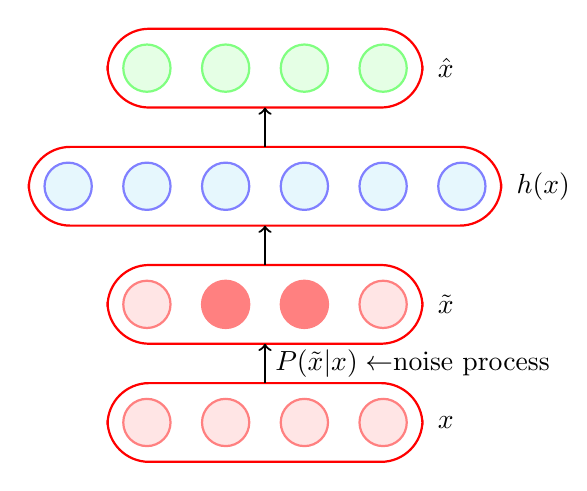
\begin{tikzpicture}
												
					\node [input_neuron] (neuron001) at (8.5,3) {};
					\node [input_neuron] (neuron002) at (9.5,3){};
					\node [input_neuron] (neuron003) at (10.5,3) {};
					\node [input_neuron] (neuron004) at (11.5,3) {};
												
					\node [input_neuron] (neuron01) at (8.5,4.5) {};
					\node [cpy_neuron] (neuron02) at (9.5,4.5){};
					\node [cpy_neuron] (neuron03) at (10.5,4.5) {};
					\node [input_neuron] (neuron04) at (11.5,4.5) {};
												
					\node [hidden_neuron] (neuron51) at (7.5,6) {} ;
					\node [hidden_neuron] (neuron52) at (8.5,6)  {};
					\node [hidden_neuron] (neuron53) at (9.5,6)  {};
					\node [hidden_neuron] (neuron54) at (10.5,6)  {};
					\node [hidden_neuron] (neuron55) at (11.5,6)  {};
					\node [hidden_neuron] (neuron56) at (12.5,6)  {};
												
					\node [output_neuron] (neuron11) at (8.5,7.5)  {};
					\node [output_neuron] (neuron12) at (9.5,7.5)  {};
					\node [output_neuron] (neuron13) at (10.5,7.5)  {};
					\node [output_neuron] (neuron14) at (11.5,7.5)  {};
												
					\node[text width=0.01cm] at (12.2,3) {$x$};
					\node[text width=0.01cm] at (12.2,4.5) {$\tilde{x}$};
					\node[text width=0.01cm] at (13.2,6) {$h(x)$};
					\node[text width=0.01cm] at (12.2,7.5) {$\hat{x}$};
												
					\draw[red!100,thick,solid,rounded corners=15pt] (8,2.5) rectangle (12,3.5);
					\draw[red!100,thick,solid,rounded corners=15pt] (8,4) rectangle (12,5);
					\draw[red!100,thick,solid,rounded corners=15pt] (7,5.5) rectangle (13,6.5);
					\draw[red!100,thick,solid,rounded corners=15pt] (8,7) rectangle (12,8);
												
					\draw[thick,->] (10,3.5) -- (10,4) node [pos=0.5,right] {$P(\tilde{x}|x) \leftarrow $noise process};
												
					\draw[thick,->] (10,5) -- (10,5.5);
												
					\draw[thick,->] (10,6.5) -- (10,7);
												
				\end{tikzpicture}
				%\end{adjustbox}
			\end{center}
		\end{overlayarea}
							
		\column{0.5\textwidth}
							
		\begin{overlayarea}{\textwidth}{\textheight}
			\begin{itemize}
				\justifying
				\item<2-> We saw this in Autoencoder
				\item<3-> We can show that for a simple input output neural network, adding Gaussian noise to the input is equivalent to weight decay ($L2$ normalizaton)
				\item<4-> Can be viewed as data augmentation
			\end{itemize}
									
		\end{overlayarea}
							
	\end{columns}
\end{frame}
% %% page 3
			
			
\begin{frame}
	\Fontvi
	% \lipsum[1]
	\begin{columns}

		\column{0.35\textwidth}
		\vspace{2em}
		\hspace{2em}
		\begin{overlayarea}{\textwidth}{\textheight}
			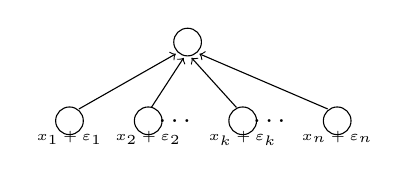
\begin{tikzpicture}
				\begin{scope}[every node/.style={sloped,allow upside down}]
					\draw (1.5,3) circle (0.5em);
					\draw (0,2) circle (0.5em)
					node[below=0.15] {\tiny $x_1 + \varepsilon_1$};
					\draw (1,2) circle (0.5em)
					node[below=0.15] {\tiny $x_2 + \varepsilon_2$}
					node[right=0.19] {\dots};
					\draw (2.2,2) circle (0.5em)
					node[below=0.15] {\tiny $x_k + \varepsilon_k$}
					node[right=0.19] {\dots};
					\draw (3.4,2) circle (0.5em) node[below=0.15] {\tiny $x_n + \varepsilon_n$};
					\draw[->] (0.12,2.15) -- (1.35,2.85);
					\draw[->] (1.04,2.17) -- (1.45,2.8);
					\draw[->] (2.12,2.17) -- (1.55,2.8);
					\draw[->] (3.28,2.15) -- (1.65,2.85);
				\end{scope}
			\end{tikzpicture}
														
			\[
				\varepsilon \sim \mathcal{N}(0,\,\sigma^{2})    
			\] 
			\vspace{-1em}
			\begin{align*}
				\onslide<2->{\widetilde{x_i} & = x_i + \varepsilon_i                                     \\}
				\onslide<3->{\widehat{y}     & = \sum_{i=1}^{n}w_i x_i                                   \\}
				\onslide<4->{\widetilde{y}   & = \sum_{i=1}^{n}w_i \widetilde{x_i}                       \\}
				\onslide<5->{                & = \sum_{i=1}^{n}w_i x_i + \sum_{i=1}^{n}w_i \varepsilon_i \\}
				\onslide<6->{                & = \widehat{y} + \sum_{i=1}^{n}w_i \varepsilon_i  }        
			\end{align*}
		\end{overlayarea}
													
		\column{0.7\textwidth}
		\vspace{1em}
		\begin{overlayarea}{\textwidth}{\textheight}
			\onslide<7->{\hspace{2em}
				We are interested in $E[(\widetilde{y} - y)^2]$}
			\begin{align*}
				\onslide<8->{E\left[(\widetilde{y} - y)^2\right] & = E\left[\Big(\widehat{y} + \sum_{i=1}^{n}w_i \varepsilon_i - y \Big)^2\right] \\}
				\onslide<9->{                                    & = E\left[\left(  \Big(\widehat{y} - y \Big)+ \Big(\sum_{i=1}^{n}w_i \varepsilon_i \Big) \right)^2\right] \\}
				\onslide<10->{                                   & = E\left[(\widehat{y} - y)^2\right] + E\left[2(\widehat{y}-y) \sum_{i=1}^{n}w_i \varepsilon_i\right] + E\left[ \Big( \sum_{i=1}^{n}w_i \varepsilon_i \Big)^2\right] \\}
				\onslide<11->{                                   & = E\left[(\widehat{y} - y)^2\right] + 0 + E\left[\sum_{i=1}^{n}w_i^2 \varepsilon_i^2\right] \\
				                                                 & \text{($\because  \varepsilon_i$ is independent of $\varepsilon_j$ and $\varepsilon_i$ is independent of ($\widehat{y}$-y) )} \\}
				\onslide<12->{                                   & = (E\left[(\widehat{y} - y)^2\right] + \highlight{\sigma^2\sum_{i=1}^{n}w_i^2} \hspace{1em} \text{(same as L2 norm penalty)}}
			\end{align*}
		\end{overlayarea}
	\end{columns}
\end{frame}
